\documentclass[a4paper,10pt]{article}
\usepackage[utf8]{inputenc}
\usepackage{graphicx}
\usepackage[section]{placeins}
\usepackage{tabularx}
\usepackage[vmargin=3cm, hmargin=2cm]{geometry}
\usepackage[T1]{fontenc}
\usepackage{specifications}
\usepackage[ngerman]{babel}

\setlength{\parskip}{2pt}

\newspec{Funktionale Anforderung}{FA}{f}
\newspec{Nicht-Funktionale Anforderungen}{NFA}{n}
\newspec{Produktdaten}{PD}{p}
\newspec{Globale Testf\"{a}lle}{T}{t}

\title{Pflichtenheft}
\author{Simon Bischof \and Jan Haag \and Adrian Herrmann \and Lin Jin \and Tobias Schlumberger \and Matthias Schnetz}

\makeindex

\begin{document}

\maketitle
\newpage
\tableofcontents
\newpage

\section{Produkt\"{u}bersicht}

%Das Produkt ist ein Werkzeug zur Analyse und Korrektheitspr\"{u}fung von Programmen. Der Benutzer hat die M\"{o}glichkeit, in eine grafische Oberfl\"{a}che ein Programm mit der im Anhang spezifizierten While-Sprache zu laden und mit Annotationen zu versehen, die als Vor- und Nachbedingungen gepr\"{u}ft werden.
Das Produkt ist ein Werkzeug zur Analyse und Korrektheitspr\"{u}fung von Programmen.

Der Benutzer interagiert \"{u}ber eine grafische Oberfläche, die neben einem Editor f\"{u}r die Erstellung und Bearbeitung von Programmen auch detaillierte R\"{u}ckmeldungen zum aktuellen Programmzustand sowie weiterf\"{u}hrende Hilfen zur Verf\"{u}gung stellt.

Nach dem Erstellen eines Programms mit der im Anhang spezifizierten While-Sprache wird dieses zunächst \"{u}bersetzt. \"{u}ber das Ergebnis dieser Analyse sowie eventuelle Fehler wird der Benutzer \"{u}ber die grafische Oberfläche informiert.

Im Anschluss entsteht nach einer Erweiterung des Quelltextes um Annahmen in Form einer definierten Annotationssprache durch den Benutzer ein beweisbares Programm, welches mit den zur Verf\"{u}gung stehenden Methoden zur Analyse des Programms untersucht werden kann.

F\"{u}r diese Zwecke bietet das Produkt sowohl eine statische als auch dynamische Pr\"{u}fung des Programmes an. Bei der dynamischen Pr\"{u}fung kann der Benutzer Eingabeparameter frei wählen und das Programm mit diesen starten. Während der Ausf\"{u}hrung werden die angegebenen Annotationen \"{u}berpr\"{u}ft. Im Fehlerfall wird das Programm im Fehlerzustand eingefroren und der Benutzer \"{u}ber die grafische Oberfläche informiert.

Bei der statischen \"{u}berpr\"{u}fung wird versucht, die Annotationen als korrekt zu beweisen. Wenn der Beweis gelingt, gibt das Programm dem Benutzer dies \"{u}ber die grafische Oberfläche bekannt; anderenfalls liefert das Programm ein Gegenbeispiel oder signalisiert, dass es keine Entscheidung treffen kann.

\section{Zielbestimmung}
\subsection{Interpreter / Run-time Checker}
\subsubsection{Musskriterien}
\begin{itemize}
  \item schrittweise Ausf\"{u}hrung eines Programms
  \item Inspektion des aktuellen Programmzustands durch den Benutzer
  \item Pr\"{u}fung von Zusicherungen in Programmen zur Laufzeit
\end{itemize}
\subsubsection{Sollkriterien}
\begin{itemize}
  \item Auswertung von Formeln mit Quantoren \"{u}ber eingeschr\"{a}nkten Bereich
\end{itemize}
\subsubsection{Kannkriterien}
\begin{itemize}
  \item Auswertung von benutzerdefinierten Ausdr\"{u}cken \"{u}ber Programmzustand
  \item Auswertung von Formeln mit Quantoren mit Hilfe eines Beweisers
  \item Breakpoints zum Halten der Ausf\"{u}hrung eines Programms an definierten Stellen
  \item Randomisiertes Testen in vorgegebenen Grenzen
\end{itemize}

\subsection{Grafische Benutzeroberfl\"{a}che}
\subsubsection{Musskriterien}
\begin{itemize}
  \item englische Sprache
  \item Steuerung der einzelnen Komponenten des Systems
  \item Anzeige von fehlgeschlagenen Laufzeitpr\"{u}fungen
  \item Speichern und Laden von Quelltexten
\end{itemize}
\subsubsection{Kannkriterien}
\begin{itemize}
  \item Syntax Highlighting
  \item Hilfe zur Syntax der While-Sprache und der Annotationssprache
  \item Markierung der aktuellen Zeile beim Halten der Ausf\"{u}hrung
\end{itemize}
\subsubsection{Abgrenzungskriterien}
\begin{itemize}
  \item Optionen, die keinen echten Mehrwert bieten
\end{itemize}

\subsection{Verifikation}
\subsubsection{Musskriterien}
\begin{itemize}
  \item formale Verifikation eines Programms mit Hilfe eines Beweisers
\end{itemize}

\subsection{While-Sprache}
\subsubsection{Musskriterien}
\begin{itemize}
  \item Zuweisungen, Bedingten Anweisungen und Schleifen
  \item Turing-Vollständigkeit
\end{itemize}
\subsubsection{Kannkriterien}
\begin{itemize}
  \item Programmiersprache unterst\"{u}tzt Methodenaufrufe
\end{itemize}
\subsubsection{Abgrenzungskriterien}
\begin{itemize}
  \item Variablentypen außer Ganzzahl, Boolean und Arrays
  \item Implementierung eines Heaps
  \item Implementierung von Nebenl\"{a}ufigkeit
  \item \"{u}berladen von Methoden
\end{itemize}

\subsection{Annotationssprache}
\subsubsection{Musskriterien}
\begin{itemize}
  \item Ausdr\"{u}cke in Annotationen \"{a}hnlich wie in der Programmiersprache, zus\"{a}tzlich Quantoren
  \item Zusicherungen erlauben Aussagen der Pr\"{a}dikatenlogik
  \item Annotationen assert und assume
\end{itemize}
\subsubsection{Sollkriterien}
\begin{itemize}
  \item syntactic sugar f\"{u}r Vor- und Nachbedingungen, (In)Varianten und globale Annahmen
\end{itemize}


\section{Produkteinsatz}
Das Produkt erm\"{o}glicht dem Benutzer die Analyse eines Programmes, das in der im Anhang beschriebenen While-Sprache geschrieben ist. Dabei ist es sowohl m\"{o}glich, die Anweisungen des Programms schrittweise oder komplett zu durchlaufen und dabei zur Laufzeit auf im Programmcode durch Annotationen eingebettete Zusicherungen zu \"{u}berpr\"{u}fen, als auch die formale Verifikation des Programms mithilfe des automatischen Theorembeweisers Z3 von Microsoft.

\subsection{Anwendungsbereiche}
\begin{itemize}
  \item Formale Verifikation von Programmen
  \item Testen von Programmen der While-Sprache
\end{itemize}

\subsection{Zielgruppen}
\begin{itemize}
  \item Softwareentwickler / Anwendungsentwickler
\end{itemize}

\subsection{Betriebsbedingungen}
\begin{itemize}
  \item \"{u}bliche Beweiserlaufzeit: 1 Stunde
  \item 
\end{itemize}

\section{Produktumgebung}
\subsection{Software}
\begin{itemize}
  \item Java Runtime Environment SE 6 oder h\"{o}her
  \item Windows NT 4.0 oder neuer oder Betriebssystem mit Wine
\end{itemize}

\subsection{Hardware}
\begin{itemize}
  \item mindestens 512 MB Arbeitsspeicher
\end{itemize}

\subsection{Schnittstellen}
\begin{itemize}
  \item Das Produkt erzeugt Dateien im SMT-LIB 2.0 Format als Schnittstelle zu Z3
\end{itemize}

\section{Funktionale Anforderungen}
%\subsection{\"{U}bersicht}
%\begin{tabular}{| l | l |}
%\hline
%/F10/ & Anzeige von Quelltext\\
%/F20/ & Syntax Highlighting\\
%/F30/ & Ver\"{a}nderung des Quelltextes\\
%/F40/ & Speichern des Quelltextes in eine Datei\\
%/F50/ & Laden eines Programms aus einer Datei\\
%/F60/ & Erkennen und Anzeigen von Syntaxfehlern\\
%/F70/ & Erkennen und Anzeigen von Typfehlern\\
%/F80/ & Ausf\"{u}hren eines Programms\\
%/F90/ & Setzen und Entfernen von Breakpoints\\
%/F100/ & Programmabbruch bei Fehler mit Anzeige des Fehlers\\
%/F110/ & Anzeige des Programmzustands\\
%/F120/ & Auswertung von benutzerdefinierten Ausdr\"{u}cken\\
%/F130/ & Auswertung der Annotationssprache\\
%/F140/ & Anzeige der Beweisereinstellungen\\
%/F150/ & Laden der Beweisereinstellungen aus einer Datei\\
%/F160/ & Speichern der Beweisereinstellungen in eine Datei\\
%/F170/ & Beweiser starten und Ergebnis anzeigen\\
%\hline
%\end{tabular}
\subsection{Details}
%GUI
\begin{FA}{Anzeige von Quelltext}{GUI!Anzeige von Quelltext}{Anzeige von Quelltext}
Der Benutzer sieht den Quelltext des aktuellen Programms in der grafischen Oberfl\"{a}che.
\end{FA}
\begin{FA}{Syntax Highlighting}{GUI!Syntax Highlighting}
Teile des angezeigten Quelltextes werden abh\"{a}ngig von ihrer Bedeutung in unterschiedlichen Farben angezeigt. \FAref{Anzeige von Quelltext}
\end{FA}
\begin{FA}{Ver\"{a}nderung des Quelltextes}{GUI!Ver\"{a}nderung des Quelltextes}
Der Benutzer kann den angezeigten Quelltext ver\"{a}ndern oder einen neuen Quelltext eingeben.
\end{FA}
\begin{FA}{Speichern des Quelltextes in eine Datei}{GUI!Speichern des Quelltextes in eine Datei}
Der Benutzer kann den eingegebenen Quelltext in eine Datei speichern. Dabei gibt der Benutzer den gew\"{u}nschten Speicherort und den Dateinamen \"{u}ber eine grafische Oberfl\"{a}che an.
\end{FA}
\begin{FA}{Laden eines Programms aus einer Datei}{GUI!Laden eines Programms aus einer Datei}
Der Benutzer kann ein Quellcode eines Programms aus einer Datei laden. Hierbei gibt der Benutzer die zu ladende Datei \"{u}ber eine grafische Oberfl\"{a}che an.
\end{FA}
\begin{FA}{Anzeigen von Syntaxfehlern}{GUI!Anzeigen von Syntaxfehlern}
Wenn der Interpreter Syntaxfehler erkannt hat (FA\FAref{Erkennen von Syntaxfehlern}), wird dies dem Benutzer angezeigt, wenn er die Programmausf\"{u}hrung oder die Beweisf\"{u}hrung anfordert.
\end{FA}
\begin{FA}{Anzeigen von Typfehlern}{GUI!Anzeigen von Typfehlern}
Wenn der Interpreter Typfehler erkannt hat (FA\FAref{Erkennen von Typfehlern}), wird dies dem Benutzer angezeigt, wenn er die Programmausf\"{u}hrung oder die Beweisf\"{u}hrung anfordert.
\end{FA}
\begin{FA}{Anzeigen von Laufzeitfehlern}{GUI!Anzeigen von Laufzeitfehlern}
Wenn bei der Ausf\"{u}hrung eines Programmes durch den Interpreter ein Fehler auftritt (FA\FAref{Anhalten des Programmablaufs bei einem Fehler}), wird dies dem Benutzer angezeigt.
\end{FA}
\begin{FA}{Setzen und Entfernen von Breakpoints}{GUI!Setzen und Entfernen von Breakpoints}
Der Benutzer kann Breakpoints zur Pausierung eines Programmdurchlaufs an Stellen des angezeigten Quellcodes setzen und wieder entfernen.
\end{FA}
\begin{FA}{Anzeige des Programmzustands}{GUI!Anzeige des Programmzustands}
Der Benutzer sieht w\"{a}hrend der Ausf\"{u}hrung eines Programms den aktuellen Inhalt aller globalen und lokalen Variablen. Die Anzeige wird nur aktualisiert, wenn das Programm die Ausf\"{u}hrung pausiert.
\end{FA}
\begin{FA}{Anhalten des Programmablaufs}{GUI!Anhalten des Programmablaufs}
Der Benutzer kann die Ausf\"{u}hrung eines Programms anhalten. Dabei wird der aktuelle Programmzustand beibehalten.
\end{FA}
\begin{FA}{Abbrechen des Programmablaufs}{GUI!Abbrechen des Programmablaufs}
Der Benutzer kann die Ausf\"{u}hrung eines Programms abbrechen. Dabei wird der Programmzustand verworfen.
\end{FA}
\begin{FA}{Anzeige von fehlgeschlagenen Annotationsbedingungen}{GUI!Anzeige von fehlgeschlagenen Annotationsbedingungen}
Meldet der Interpreter eine fehlgeschlagene Annotationsbedingung (FA\FAref{Auswertung der Ausdr\"{u}cke der Annotationssprache}), so wird dies dem Benutzer angezeigt.
\end{FA}
\begin{FA}{Eingabe von benutzerdefinierten Ausdr\"{u}cken}{GUI!Eingabe von benutzerdefinierten Ausdr\"{u}cken}
Der Benutzer kann während der angehaltenen Ausf\"{u}hrung eines Programms Ausdr\"{u}cke eingeben, die vom Interpreter ausgewertet werden und deren Ergebnis dem Benutzer angezeigt wird.
\end{FA}
\begin{FA}{Anzeige der Beweisereinstellungen}{GUI!Anzeige der Beweisereinstellungen}
Der Benutzer kann die aktuellen Einstellungen (\PDref{Benutzereinstellungen}) f\"{u}r die Ausf\"{u}hrung des Beweisers (siehe FA\FAref{Starten}) anzeigen lassen. Diese werden vor der Anzeige aus einer Datei geladen (FA\FAref{Laden der Beweisereinstellungen aus einer Datei}) und bei einer Ver\"{a}nderung wieder in eine Datei geschrieben (FA\FAref{Speichern der Beweisereinstellungen in eine Datei}).
\end{FA}
\begin{FA}{Laden der Beweisereinstellungen aus einer Datei}{GUI!Laden der Beweisereinstellungen aus einer Datei}
Die Einstellungen f\"{u}r die Ausf\"{u}hrung des Beweisers (siehe PD\PDref{Benutzereinstellungen}) werden automatisch aus einer Datei gelesen.
\end{FA}
\begin{FA}{Speichern der Beweisereinstellungen in eine Datei}{GUI!Speichern der Beweisereinstellungen in eine Datei}
Die Einstellungen (siehe PD\PDref{Benutzereinstellungen}) werden in eine Datei gespeichert.
\end{FA}
\begin{FA}{Starten des Beweisvorgangs}{GUI!Starten des Beweisvorgangs}
Der Benutzer kann den Beweisvorgang mit Hilfe des Beweisers unter den eingegebenen Einstellungen starten.
\end{FA}
\begin{FA}{Anzeige des Ergebnis des Beweisers}{GUI!Anzeige des Ergebnis des Beweisers}
Nach dem Durchlauf des Beweisers wird dem Benutzer das Ergebnis des Beweisvorgangs angezeigt.
\end{FA}

%Interpreter
\begin{FA}{Erkennen von Syntaxfehlern}{Interpreter!Erkennen von Syntaxfehlern}
Der Interpreter erkennt Syntaxfehler des eingegebenen Quelltextes.
\end{FA}
\begin{FA}{Erkennen von Typfehlern}{Interpreter!Erkennen von Typfehlern}
Der Interpreter erkennt Typfehler des eingegebenen Quelltextes.
\end{FA}
\begin{FA}{Ausf\"{u}hren eines Programms}{Interpreter!Ausf\"{u}hren eines Programms}
Die Anweisungen im aktuell angezeigten Quelltext k\"{o}nnen ausgef\"{u}hrt werden. Dabei sind folgende Ausf\"{u}hrungsmodi m\"{o}glich:\\
\begin{tabularx}{0.85\textwidth}{lX}
\leftskip=0.1\textwidth
Single Step & Es wird auf eine Interaktion des Benutzers nur eine Anweisung ausgef\"{u}hrt.\\
Run until Breakpoint & Es werden sequentiell alle Anweisungen ausgef\"{u}hrt, bis das Programm beendet ist oder ein Breakpoint (FA\FAref{Setzen und Entfernen von Breakpoints}) erreicht wird.\\
\end{tabularx}
\end{FA}
\begin{FA}{Anhalten des Programmablaufs bei einem Fehler}{Interpreter!Anhalten des Programmablaufs bei einem Fehler}
Tritt ein Fehler zur Laufzeit des Programms auf, wird die Ausf\"{u}hrung abgebrochen und der Fehler dem Benutzer angezeigt.
\end{FA}
\begin{FA}{Auswertung von benutzerdefinierten Ausdr\"{u}cken}{Interpreter!Auswertung von benutzerdefinierten Ausdr\"{u}cken}
Der Benutzer kann Ausdr\"{u}cke \"{u}ber den aktuellen Programmzustand auswerten lassen.
\end{FA}
\begin{FA}{Auswertung der Ausdr\"{u}cke der Annotationssprache}{Interpreter!Auswertung der Ausdr\"{u}cke der Annotationssprache}
W\"{a}hrend der Programmausf\"{u}hrung werden die Bedingungen der Annotationssprache ausgewertet. Schl\"{a}gt eine \"{U}berpr\"{u}fung fehl, so wird die Ausf\"{u}hrung des Programms angehalten und dem Benutzer angezeigt, welche Bedingung falsch ist.
\end{FA}

%Beweiser
\begin{FA}{Beweiservorgang durchf\"{u}hren}{Beweiser!Beweisvorgang durchf\"{u}hren}
Der Beweisvorgang f\"{u}r das aktuelle Programm wird durchgef\"{u}hrt.
\end{FA}

\section{Produktdaten}
Es sind folgende Daten des Benutzers zu Speichern:\\
\begin{PD}{Benutzereinstellungen}{Benutzereinstellungen}{Benutzereinstellungen}
\begin{itemize}
  \item Timeout in Sekunden f\"{u}r den Beweiser
  \item Speicherbegrenzung in Megabyte f\"{u}r den Beweiser
\end{itemize}
\end{PD}
\begin{PD}{Zuletzt ge\"{o}ffnetes Verzeichnis}{Zuletzt ge\"{o}ffnetes Verzeichnis}{Zuletzt ge\"{o}ffnetes Verzeichnis}
\begin{itemize}
  \item Das zuletzt durch \FAref{Laden eines Programms aus einer Datei} ge\"{o}ffnete Verzeichnis.
\end{itemize}
\end{PD}

\section{Produktleistungen}
\begin{itemize}
  \item Verifikation- und Falsifikationsr\"{u}ckmeldungen vom Beweiser bezüglich der Spezifikation m\"{u}ssen korrekt sein, in anderen F\"{a}llen soll dem Benutzer mitgeteilt werden, dass der Beweiser das Problem nicht l\"{o}sen kann
  \item Interpreter: Anweisungen mit weniger als 50 Operatoren werden in weniger als 0,1 Sekunde ausgeführt
  \item Parser: Programme mit 10.000 Zeilen werden in weniger als 1 Sekunde geparst
  \item vollständige Dokumentation der Syntax der While- und Annotationssprache
\end{itemize}

\section{Weitere nichtfunktionale Anforderungen}
Die Lizenz von Z3 erlaubt ausschlie\ss{}lich eine nicht-kommerzielle Benutzung.

\section{Qualit\"{a}tsanforderungen}
\begin{itemize}
  \item Programmiersprache muss erweiterbar sein
  \item m\"{o}gliche Anbindung anderer Beweiser, die das SMT-LIB 2.0 Format unterst\"{u}tzen
  \item unter (durch benutzerdefinierte Einstellungen vorgegebene, FA\FAref{Anzeige der Beweisereinstellungen}) Normalbedingungen st\"{u}rzt das Produkt nicht ab
  \item jede Aktion gibt in jedem Fall eine R\"{u}ckmeldung an den Benutzer
\end{itemize}

\section{Globale Testf\"{a}lle und Testszenarien}
Folgende Funktionssequenzen sind zu \"{u}berpr\"{u}fen:\\
%\begin{description}
%\end{T}
\begin{T}{}{}Eingabe des leeren Programms $\to$ keine Syntaxfehler
\end{T}\begin{T}{}{}Eingabe des leeren Programms ohne Annotationen, Beweisvorgang starten $\to$ Verifikation durch den Beweiser
\end{T}\begin{T}{}{}Eingabe des leeren Programms, Annotation \texttt{ensure false}, Programmausf\"{u}hrung $\to$ Annotationsbedingung schl\"{a}gt fehl
\end{T}\begin{T}{}{}Eingabe des leeren Programms, Annotation \texttt{ensure true}, Programmausf\"{u}hrung $\to$ Annotationsbedingung schl\"{a}gt nicht fehl
\end{T}\begin{T}{}{}Eingabe eines beliebigen Programms, Annotation \texttt{require false}, Programmausf\"{u}hrung $\to$ Annotationsbedingung schl\"{a}gt fehl, Programmausf\"{u}hrung wird abgebrochen
\end{T}\begin{T}{}{}Eingabe eines Programms mit Zuweisung \texttt{x = 1}, Annotation \texttt{require x>0}, Programmausf\"{u}hrung $\to$ Annotationsbedingung schl\"{a}gt nicht fehl
\end{T}\begin{T}{}{}Eingabe eines Programms mit Syntaxfehler (z.B. fehlerhafte Klammerung, fehlendes Semikolon, Methodenname ist Keyword) $\to$ Anzeige des Syntaxfehlers
\end{T}\begin{T}{}{}Eingabe eines Programms mit while-Schleife oder if-Konstrukt, deren Bedingung kein boolean ist $\to$ Anzeige des Typfehlers
\end{T}\begin{T}{}{}Eingabe eines Programms mit einem Operator, der nur auf Ganzzahlen definiert ist und auf einen boolean angewendet wird $\to$ Anzeige des Typfehlers
\end{T}\begin{T}{}{}Eingabe eines Programms mit einem Operator, der nur auf booleans definiert ist und auf Ganzzahlen angewendet wird $\to$ Anzeige des Typfehlers
\end{T}\begin{T}{}{}Eingabe eines Programms mit einer Zuweisung eines boolean an eine Ganzzahl $\to$ Anzeige des Typfehlers
\end{T}\begin{T}{}{}Eingabe eines Programms mit einer Zuweisung einer Ganzzahl an einen boolean $\to$ Anzeige des Typfehlers
\end{T}\begin{T}{}{}Eingabe eines Programms mit einer Zuweisung einer Ganzzahl oder eines boolean an ein Array $\to$ Anzeige des Typfehlers
\end{T}\begin{T}{}{}Eingabe eines Programms mit einem Vergleichsoperator, der auf zwei unterschiedliche Typen ausgef\"{u}hrt wird $\to$ Anzeige des Typfehlers
\end{T}\begin{T}{}{}Eingabe eines Programms mit Zuweisung \texttt{y = 2x}, Annotation \texttt{ensure y==2x}, Beweisvorgang starten $\to$ Verifizierung durch den Beweiser
\end{T}\begin{T}{}{}Eingabe eines Programms mit Zuweisung \texttt{y = 2x}, Annotation \texttt{ensure y\%2==0}, Beweisvorgang starten $\to$ Verifizierung durch den Beweiser
\end{T}\begin{T}{}{}Eingabe eines l\"{a}ngeren Programms ohne Schleifen und ohne if-Konstrukt, Eingabe von Annotationen, die in jedem Fall wahr sind, Beweisvorgang starten $\to$ Verifizierung durch den Beweiser
\end{T}\begin{T}{}{}Eingabe eines l\"{a}ngeren Programms ohne Schleifen und mit if-Konstrukt, Eingabe von Annotationen, die in jedem Fall wahr sind, Beweisvorgang starten $\to$ Verifizierung durch den Beweiser
\end{T}\begin{T}{}{}Eingabe eines l\"{a}ngeren Programms mit Schleifen, Eingabe von Annotationen, die in jedem Fall wahr sind, Beweisvorgang starten $\to$ Verifizierung durch den Beweiser
\end{T}\begin{T}{}{}Eingabe eines Programms mit Annotation \texttt{ensure x!=x}, Beweisvorgang starten $\to$ Falsifikation durch den Beweiser
\end{T}\begin{T}{}{}Eingabe eines l\"{a}ngeren Programms mit Schleife (z.B. russische Multiplikation, Maximum der Zahlen in einem Array), Eingabe von Annotationen, die in mindestens einem Fall falsch sind, Beweisvorgang starten $\to$ Falsifikation durch den Beweiser
\end{T}\begin{T}{}{}Eingabe eines Programms mit Annotation \texttt{require x\%2==0}, Zuweisung \texttt{y = 2*(x/2)} und Annotation \texttt{ensure (x==y)}, Beweisvorgang starten $\to$ Verifikation durch den Beweiser
\end{T}\begin{T}{}{}Eingabe eines Programms mit Division durch 0, Ausf\"{u}hrung des Programms $\to$ Anzeige des Laufzeitfehlers
\end{T}\begin{T}{}{}Eingabe eines Programms mit Deklaration und Initialisierung eines Arrays, fehlerhafter Arrayzugriff, Ausf\"{u}hrung des Programms$\to$ Anzeige des Laufzeitfehlers
\end{T}
%\end{description}

\section{Systemmodelle}
\subsection{Komponenten\"{u}bersicht}
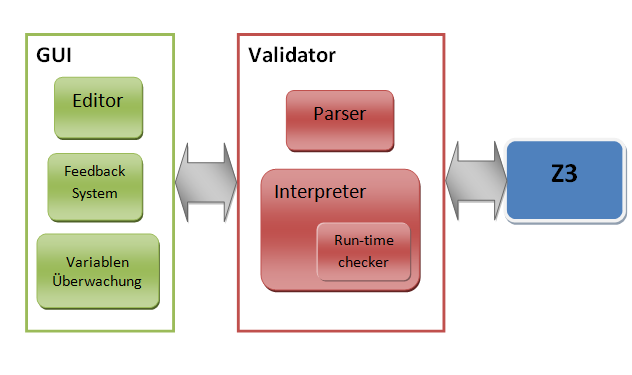
\includegraphics[width=\textwidth]{images/overview.png}
\subsection{Workflow}
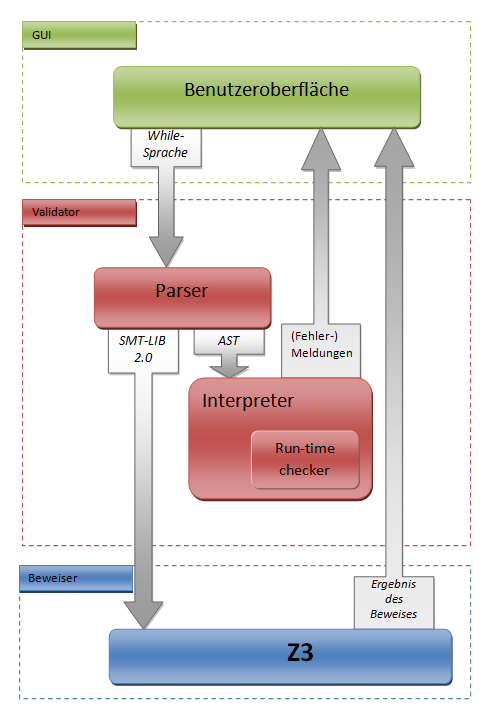
\includegraphics[width=\textwidth]{images/process.png}

\section{Benutzeroberfl\"{a}che}
\subsection{Übersicht}
\begin{figure}[h!]
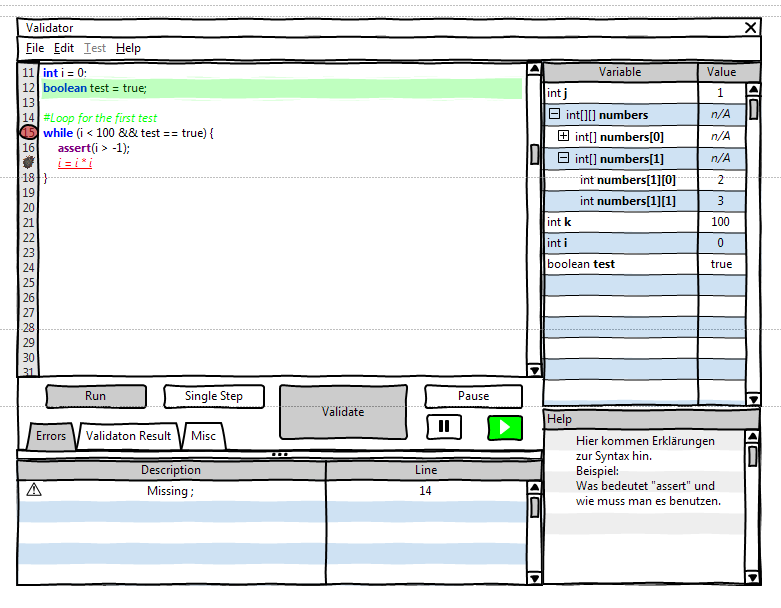
\includegraphics[width=\textwidth]{images/mockupf.png}
\end{figure}
\subsection{Menüpunkte}
\begin{figure}[h!]
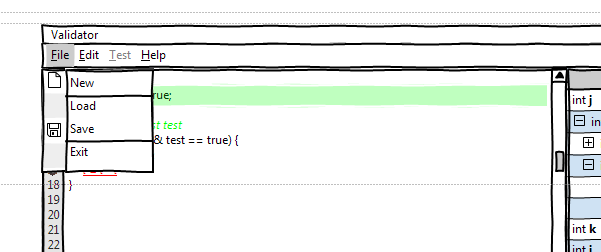
\includegraphics[width=\textwidth]{images/menu1.png}
\end{figure}
\begin{figure}[h!]
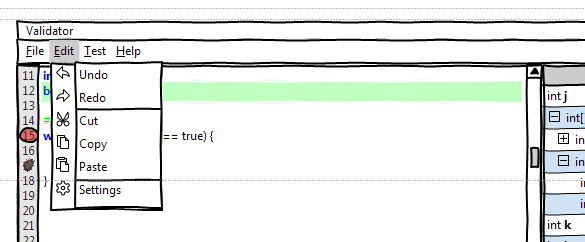
\includegraphics[width=\textwidth]{images/menu2.png}
\end{figure}
\begin{figure}[h!]
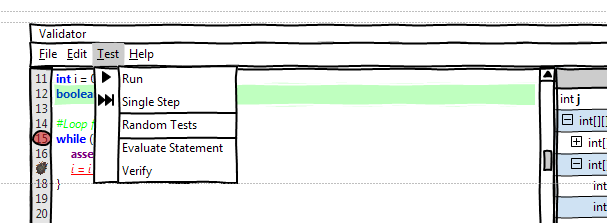
\includegraphics[width=\textwidth]{images/menu3.png}
\end{figure}
\begin{figure}[h!]
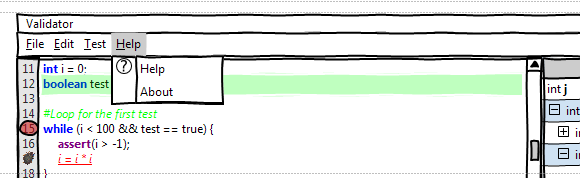
\includegraphics[width=\textwidth]{images/menu4.png}
\end{figure}

\section{Spezielle Anforderungen an die Entwicklungsumgebung}
\begin{description}
  \item[Versionsverwaltung] Git (GitHub)
  \item[Kommunikation] E-Mail, GitHub Wiki
  \item[Dokumente] \LaTeXe
  \item[Programmiersprache] Java
  \item[UML-Diagramme] Dia, SD Edit (für Sequenzdiagramme)
  \item[Entwicklungsumgebung] keine einheitliche, Ausschluss entwicklungsumgebungsspezifischer Dateien durch .gitignore
\end{description}

\section{Zeit- und Ressourcenplanung}
\subsection{Projektplan}
\begin{tabular}[h]{| l | l |}
\textbf{Komponente} & \textbf{Zeit}\\
\hline
GUI & 75 Stunden\\
Parser & 75 Stunden\\
Interpreter & 75 Stunden\\
Run-time Checker & 100 Stunden\\
Typchecker & 75 Stunden\\
Beweiseranbindung & 100 Stunden\\
\end{tabular}
\subsection{Phasenverantwortliche}
\begin{tabular}[h]{| l | r |}
\hline
\textbf{Phase} & \textbf{Verantwortliche(r)}\\
\hline
Pflichtenheft & Tobias\\
\hline
Entwurf & Adrian\\
\hline
Implementierung & Simon, Jan\\
\hline
Validierung & Lin\\
\hline
Abschlusspr\"{a}sentation & Matthias\\
\hline
\end{tabular}


\section{Erg\"{a}nzungen}
\subsection{While-Sprache}
\subsubsection{Variablentypen}
\begin{description}
\item[Ganzzahl] ganze Zahl beliebiger Genauigkeit.
\item[Boolean] Wahrheitswert, entweder wahr oder falsch.
\item[Array] eine Zusammenfassung mehrerer Variablen eines Variablentyps. Die maximale Anzahl m\"{o}glicher Variablen in einem Array ist nach erster Festlegung konstant.
\end{description}
\subsubsection{Sprachkonstrukte}
\begin{tabularx}{\textwidth}{| l | X |}
\hline
\textbf{Konstrukt} & \textbf{Bedeutung}\\
\hline
sequentelle Komposition & Hintereinanderausführung von Anweisungen.\\
\hline
if-else & Ausf\"{u}hrung bestimmter Anweisungen, falls eine Bedingung erf\"{u}llt ist. Ausf\"{u}hrung anderer Anweisungen, falls die Bedingung nicht erf\"{u}llt ist.\\
\hline
while & Wiederholte Ausf\"{u}hrung von bestimmten Anweisungen, wenn eine Bedingung erf\"{u}llt ist.\\
\hline
Methoden & Definition einer Folge von Anweisungen mit Parametern, die zu einem anderen Zeitpunkt im Programmablauf aufgerufen werden k\"{o}nnen, und einen Wert zur\"{u}ckgeben.\\
\hline
einzeilige Kommentare & Annotation, die keinen Einfluss auf die Quelltextverarbeitung haben.\\
\hline
Deklaration & Festlegung von Eigenschaften (Variablentyp, Bezeichner, \ldots) von Variablen und Methoden.\\
\hline
\end{tabularx}
\subsubsection{Operatoren}
\begin{tabularx}{\textwidth}{| l | X | l | X |}
\hline
\textbf{Operator} & \textbf{Eingabetypen} & \textbf{Ergebnistyp} & \textbf{Funktion}\\
\hline
\texttt{==} & 2 Variablen desselben Typs & Boolean & Pr\"{u}ft \texttt{T1} und \texttt{T2} auf Gleichheit, falls sie vom selben Variablentyp sind. Arrays sind gleich, wenn alle Elemente der tiefsten Ebene des Arrays gleich sind.\\
\texttt{!=} & 2 Variablen desselben Typs & Boolean & Pr\"{u}ft \texttt{T1} und \texttt{T2} auf Ungleichheit, falls sie vom selben Variablentyp sind. Liefert denselben Wert wie die Negation von \texttt{==}.\\
\texttt{=} & 1 Variable und ein Ausdruck & ? & Weist der Variable den Wert des Ausdrucks zu, wenn dieser Wert vom selben Variablentyp ist, wie die Variable.\\
\hline
\texttt{<} & 2 Ganzzahlen, \texttt{Ganzzahl1} und \texttt{Ganzzahl2} & Boolean & Pr\"{u}ft, ob \texttt{Ganzzahl1} kleiner als \texttt{Ganzzahl2} ist.\\
\texttt{>} & 2 Ganzzahlen, \texttt{Ganzzahl1} und \texttt{Ganzzahl2} & Boolean & Pr\"{u}ft, ob \texttt{Ganzzahl1} gr\"{o}\ss{}er als \texttt{Ganzzahl2} ist.\\
\texttt{<=} & 2 Ganzzahlen, \texttt{Ganzzahl1} und \texttt{Ganzzahl2} & Boolean & Pr\"{u}ft, ob \texttt{Ganzzahl1} kleiner oder gleich \texttt{Ganzzahl2} ist.\\
\texttt{>=} & 2 Ganzzahlen, \texttt{Ganzzahl1} und \texttt{Ganzzahl2} & Boolean & Pr\"{u}ft, ob \texttt{Ganzzahl1} gr\"{o}\ss{}er oder gleich \texttt{Ganzzahl2} ist.\\
\texttt{+} & 1 Ganzzahl, \texttt{Ganzzahl} & Ganzzahl & Gibt \texttt{Ganzzahl} zur\"{u}ck.\\
\texttt{-} & 1 Ganzzahl, \texttt{Ganzzahl} & Ganzzahl & Gibt -\texttt{Ganzzahl} zur\"{u}ck.\\
\texttt{+} & 2 Ganzzahlen, \texttt{Ganzzahl1} und \texttt{Ganzzahl2} & Ganzzahl & Addiert \texttt{Ganzzahl1} und \texttt{Ganzzahl2}.\\
\texttt{-} & 2 Ganzzahlen, \texttt{Ganzzahl1} und \texttt{Ganzzahl2} & Ganzzahl & Subtrahiert \texttt{Ganzzahl2} von \texttt{Ganzzahl1}.\\
\texttt{*} & 2 Ganzzahlen, \texttt{Ganzzahl1} und \texttt{Ganzzahl2} & Ganzzahl & Multipliziert \texttt{Ganzzahl1} mit \texttt{Ganzzahl2}.\\
\texttt{/} & 2 Ganzzahlen, \texttt{Ganzzahl1} und \texttt{Ganzzahl2} & Ganzzahl & Dividiert \texttt{Ganzzahl1} durch \texttt{Ganzzahl2}. Das Ergebnis wird zur Null hin gerundet.\\
\texttt{\%} & 2 Ganzzahlen, \texttt{Ganzzahl1} und \texttt{Ganzzahl2} & Ganzzahl & Liefert den Rest der Ganzzahldivision von \texttt{Ganzzahl1} durch \texttt{Ganzzahl2}.\\
\hline
\texttt{!} & 1 Boolean, \texttt{Boolean} & Boolean & Negiert den Wert von \texttt{Boolean}.\\
\texttt{\&} & 2 Boolean, \texttt{Boolean1} und \texttt{Boolean2} & Boolean & Liefert die Konjunktion von \texttt{Boolean1} und \texttt{Boolean2}.\\
\texttt{|} & 2 Boolean, \texttt{Boolean1} und \texttt{Boolean2} & Boolean & Liefert die Disjunktion von \texttt{Boolean1} und \texttt{Boolean2}.\\
\hline
\end{tabularx}
\subsubsection{Sonstige Spracheigenschaften}
\begin{itemize}
  \item Lexical Scoping
  \item Kurzauswertung von logischen Operatoren
\end{itemize}

\subsection{Annotationssprache}
Die Annotationssprache besteht aus Ausdr\"{u}cken der While-Sprache mit Quantoren und zus\"{a}tzlich den folgenden Konstrukten:\\
\begin{tabularx}{\textwidth}{| l | X |}
\hline
\texttt{require} & Stellt eine Vorbedingung vor Schleifen oder Methoden dar.\\
\texttt{ensure} & Stellt eine Nachbedingung nach Schleifen oder Methoden dar.\\
\texttt{assert} & Stellt eine Bedingung an der aktuellen Stelle im Programmablauf dar.\\
\texttt{assume} & Stellt eine globale, als wahr angenommene Aussage dar.\\
\texttt{invariant} & Stellt eine Invariante einer Schleife dar.\\
\hline
\texttt{thereis} & Existenzquantor $\exists$\\
\texttt{forall} & Allquantor $\forall$\\
\hline
\end{tabularx}


\section{Glossar}
\begin{description}
\item[Anweisung (Programm)] Eine syntaktisch korrekte Vorschrift, die bei der Abarbeitung des Programms auszuf\"{u}hren ist.
\item[Beweiser] Ein Programm, das versucht die G\"{u}ltigkeit eines Theorems zu \"{u}berpr\"{u}fen. Ein Beispiel f\"{u}r ein solches Programm ist $\to$Z3.
\item[Kurzauswertung] Die Auswertung eines Ausdrucks wird abgebrochen, sobald der Wert des Ausdrucks bekannt ist.
\item[Lexical Scoping] Auf eine lokale Variable kann nur in ihrem lexikalischen Sichtbarkeitsbereich Bezug genommen werden.
\item[sequentielle Komposition] Hintereinanderausf\"{u}hrung von mehreren Anweisungen.
\item[SMT-LIB 2.0] Ein Standardformat zur Beschreibung von Satisfiability Modulo Theories Problemen, d.h. Formeln der Pr\"{a}dikatenlogik erster Stufe.
\item[Z3] Ein $\to$Beweiser von Microsoft.
\end{description}

\printindex[FA]
%\printindex[PD]
%\printindex[T]

\end{document}
